\chapter{Quantum Electrodynamics}
\label{Quantum Electrodynamics}

In this chapter, we will define the interaction Hamiltonian of Quantum Electrodynamics (QED), describing the photon mediated electromagnetic interaction between electrically charged fermions, and we will derive the composition of the corresponding dressed particles.

\section{Electric charge operator}
\label{Electric charge operator}

On each point $\n$ of space, the electric charge operator is defined by:
\begin{equation*}
\Qop \n \eqdef \e \sum_{\pt,\sp',\sp} \Qp \pt \left( \SCop \pt \n {\sp'} + \SAop {\antiparticle \pt} \n {\sp'} \right) \gammat 0 \left( \SAop \pt \n \sp + \SCop {\antiparticle \pt} \n \sp \right)
\end{equation*}
where $\e$ is the elementary electric charge (opposite electric charge of a bare electron) and $\Qp \pt$ the electric charge number of fermions of type $\pt$: $\Qp \pt = 0$ for the neutrinos $\pt \in \{ \neutrinoelectron, \neutrinomuon, \neutrinotauon \}$, $\Qp \pt = -1$ for the charged leptons $\pt \in \{ \electron, \muon, \tauon \}$, $\Qp \pt = \frac 2 3$ for the quarks $\pt \in \{ \quarkup, \quarkcharm, \quarktop \}$ and $\Qp \pt = - \frac 1 3$ for the quarks $\pt \in \{ \quarkdown, \quarkstrange, \quarkbottom \}$. In this expression, the creation and annihilation spinor operators are defined as in appendix \ref{Dirac spinors} and the Dirac matrices as in appendix \ref{Dirac matrices}.

The anti-particle creation and annihilation spinor operators in this expression yield to a uniformly distributed mean electric charge in the vacuum state, given by:
\begin{equation*}
\bra \vac \Qop \n \ket \vac = \e \sum_{\pt,\sp} \Qp \pt = - 4 \e
\end{equation*}
and called `zero-point electric charge'. Since this charge distribution is uniform, it doesn't have any contribution to the interaction Hamiltonian as defined in section \ref{QED interaction Hamiltonian}.

\section{Electric current operator}

On each point $\n$ of space, the electric current operator is defined by:
\begin{equation*}
\Jop \n \eqdef \e \c \sum_{\pt,\sp',\sp} \Qp \pt \left( \SCop \pt \n {\sp'} + \SAop {\antiparticle \pt} \n {\sp'} \right) \gamvec \left( \SAop \pt \n \sp + \SCop {\antiparticle \pt} \n \sp \right)
\end{equation*}
where the summation goes over all fermions $\pt$. In this expression too, the creation and annihilation spinor operators are defined as in appendix \ref{Dirac spinors} and the Dirac matrices as in appendix \ref{Dirac matrices}.

\section{Electric potential operator}

On each point $\n$ of space, the electric potential operator is defined by:
\begin{equation*}
\Vop \n \eqdef \sum_{\n'} \frac{\Qop {\n'}}{8 \pi \vpty \a} ( 1 + 2 \N )^{-3} \sum_{\q_\photon \neq \sv 0} \frac{\exp{\i 2 \pi \q_\photon \ssp ( \n - \n' )}}{\pi q_\photon^2}
\end{equation*}
where $\vpty$ is the permittivity of the bare vacuum. Its constant Fourier component has been set to $0$ (which is consistent with the Coulomb gauge condition used in appendix \ref{Photon spinors}), so that the zero-point electric charge in section \ref{Electric charge operator} doesn't have any contribution to the interaction Hamiltonian as defined in section \ref{QED interaction Hamiltonian}.

\section{Magnetic potential operator}

On each point $\n$ of space, the magnetic potential operator is defined by:
\begin{equation*}
\Aop \n \eqdef \sum_{\sp_\photon} \tSCop \photon \n {\sp_\photon} + \tSAop \photon \n {\sp_\photon}
\end{equation*}
In this expression, the creation and annihilation spinor operators are defined as in appendix \ref{Photon spinors}.

\section{QED interaction Hamiltonian}
\label{QED interaction Hamiltonian}

The interaction Hamiltonian of QED is defined by:
\begin{equation*}
\HopQED \eqdef \sum_{\n} \Jop \n \ssp \Aop \n + \Qop \n \Vop \n
\end{equation*}
Its development on the plane waves basis is given by:
\begin{eqnarray*}
\sum_{\n} \Jop \n \ssp \Aop \n & = & \sqrt{\frac{\e^2 \h \c}{8 \pi^2 \vpty \a^2}} ( 1 + 2 \N )^{-3/2} \sum_{\pt, \q, \sp', \sp} \Qp \pt \sum_{\q_\photon \neq \sv 0, \sp_\photon} q_\photon^{-1/2} \\
&& \left[ \left( \SCop \pt {\q - \q_\photon} {\sp'} + \SAop {\antiparticle \pt} {-\q + \q_\photon} {\sp'} \right) \gamvec \left( \SAop \pt \q \sp + \SCop {\antiparticle \pt} {-\q} \sp \right) \ssp \right. \\
&& \cphotonspin {\q_\photon} {\sp_\photon} \cop \photon {\q_\photon} {\sp_\photon} \sqrt{1 + \Nop \photon {\q_\photon} {\sp_\photon}} + \\
&& \left( \SCop \pt {\q + \q_\photon} {\sp'} + \SAop {\antiparticle \pt} {-\q - \q_\photon} {\sp'} \right) \gamvec \left( \SAop \pt \q \sp + \SCop {\antiparticle \pt} {-\q} \sp \right) \ssp \\
&& \left. \photonspin {\q_\photon} {\sp_\photon} \aop \photon {\q_\photon} {\sp_\photon} \sqrt{\Nop \photon {\q_\photon} {\sp_\photon}} \right]
\end{eqnarray*}
\begin{eqnarray*}
\sum_{\n} \Qop \n \Vop \n & = & \frac{\e^2}{8 \pi^2 \vpty \a} ( 1 + 2 \N )^{-3} \sum_{\pt,\q,\sp',\sp} \Qp \pt \sum_{\pt_0,\q_0,\sp'_0,\sp_0} \Qp {\pt_0} \sum_{\q_\photon \neq \sv 0} q_\photon^{-2} \\
&& \left( \SCop \pt {\q + \q_\photon} {\sp'} + \SAop {\antiparticle \pt} {-\q - \q_\photon} {\sp'} \right) \gammat 0 \left( \SAop \pt \q \sp + \SCop {\antiparticle \pt} {-\q} \sp \right) \\
&& \left( \SCop {\pt_0} {\q_0 - \q_\photon} {\sp'_0} + \SAop {\antiparticle {\pt_0}} {-\q_0 + \q_\photon} {\sp'_0} \right) \gammat 0 \left( \SAop {\pt_0} {\q_0} {\sp_0} + \SCop {\antiparticle {\pt_0}} {-\q_0} {\sp_0} \right)
\end{eqnarray*}

\section{Dressed states}

As a consequence of the electromagnetic interaction between the photon and the charged fermion fields, an excitation of a single particle field like $\ketQ N \pt \q \sp$ is unstable and is also a poor model for observed particles. In fact, these particles are always being observed ``dressed'', \textit{i.e.} forming a particle complex together with excitations of the other fields. As a consequence, the ``bare'' rest mass, electric charge and magnetic moment of these particles, as they appear in the QED model, do not correspond to the values observed by dressed particles. These renormalized values as well as the composition of dressed particles can be calculated in the frame of QED as a function of the bare values, which can also be indirectly determined experimentally.

We consider a bare state of the form $\ket{{\bFQ N \pt \q \sp}_0}$ and will derive the corresponding dressed state $\ket{\Psi}$ as eigenstate of $\Hop_0 + \Hop'$ for an eigenvalue $E$ to be determined. Assuming the bare and dressed states aren't orthogonal to each other, we write the latter as:
\begin{equation*}
\ket{\Psi} \eqdef \FT \Psi \left( {\bFQ N \pt \q \sp}_0 \right) \sum_{\bFQ N \pt \q \sp} \FT \Phi_0 \left( \bFQ N \pt \q \sp \right) \ket{\bFQ N \pt \q \sp}
\end{equation*}
using unnormalized coefficients $\FT \Phi_0$ verifying the condition:
\begin{equation*}
\FT \Phi_0 \left( {\bFQ N \pt \q \sp}_0 \right) = 1
\end{equation*}
The eigenvalue equation, projected on $\ket{{\bFQ N \pt \q \sp}_0}$ resp. on another plane wave state $\ket{{\bFQ N \pt \q \sp}_1}$, reads:
\begin{eqnarray*}
H'_{0,0} + \sum_{{\bFQ N \pt \q \sp}_2 \neq {\bFQ N \pt \q \sp}_0} H'_{0,2} \FT \Phi_{2,0} & = & E - E_0 \\
H'_{1,0} + \sum_{{\bFQ N \pt \q \sp}_2 \neq {\bFQ N \pt \q \sp}_0} H'_{1,2} \FT \Phi_{2,0} & = & ( E - E_1 ) \FT \Phi_{1,0}
\end{eqnarray*}
where we use the shorthand notations:
\begin{eqnarray*}
H'_{b,a} & \eqdef & \bra{{\bFQ N \pt \q \sp}_b} \Hop' \ket{{\bFQ N \pt \q \sp}_a} \\
E_a & \eqdef & \bra{{\bFQ N \pt \q \sp}_a} \Hop_0 \ket{{\bFQ N \pt \q \sp}_a} \\
\FT \Phi_{a,0} & \eqdef & \FT \Phi_0 \left( {\bFQ N \pt \q \sp}_a \right)
\end{eqnarray*}
To solve this equation iteratively, we develop $\Hop'$, $\FT \Phi_0$ and $E$ as power series in the elementary electric charge $\e$:
\begin{eqnarray*}
\Hop' & \eqdef & \Hop'^{(1)} + \Hop'^{(2)} \\
\FT \Phi_0 & \eqdef & \sum_{n=0}^\infty \FT \Phi_0^{(n)} \\
E & \eqdef & \sum_{n=0}^\infty E^{(n)}
\end{eqnarray*}
where we take:
\begin{eqnarray*}
\Hop'^{(1)} & \eqdef & \sum_{\n} \Jop \n \ssp \Aop \n \\
\Hop'^{(2)} & \eqdef & \sum_{\n} \Qop \n \Vop \n \\
\FT \Phi_{a,0}^{(0)} & \eqdef & \delta_{a,0}
\end{eqnarray*}
In the case of bare states which are nondegenerate with respect to $\Hop_0$, \textit{i.e.} such as $E_2 \neq E_0$ for any ${\bFQ N \pt \q \sp}_2 \neq {\bFQ N \pt \q \sp}_0$, assuming that the eigenvalue equation should hold to each order separately, we have to the zeroth order:
\begin{equation*}
E^{(0)} = E_0
\end{equation*}
to the first order:
\begin{eqnarray*}
E^{(1)} & = & H'^{(1)}_{0,0} \\
\FT \Phi_{1,0}^{(1)} & = & \frac{H'^{(1)}_{1,0}}{E_0 - E_1}
\end{eqnarray*}
to the second order:
\begin{eqnarray*}
E^{(2)} & = & H'^{(2)}_{0,0} + \sum_{{\bFQ N \pt \q \sp}_2 \neq {\bFQ N \pt \q \sp}_0} \frac{H'^{(1)}_{0,2} H'^{(1)}_{2,0}}{E_0 - E_2} \\
\FT \Phi_{1,0}^{(2)} & = & \frac{H'^{(2)}_{1,0}}{E_0 - E_1} + \sum_{{\bFQ N \pt \q \sp}_2 \neq {\bFQ N \pt \q \sp}_0} \frac{H'^{(1)}_{1,2} H'^{(1)}_{2,0}}{( E_0 - E_1 ) ( E_0 - E_2 )} - \frac{H'^{(1)}_{1,0} H'^{(1)}_{0,0}}{( E_0 - E_1 )^2}
\end{eqnarray*}
and to the order $n > 2$:
\begin{eqnarray*}
E^{(n)} & = & \sum_{{\bFQ N \pt \q \sp}_2 \neq {\bFQ N \pt \q \sp}_0} \left( H'^{(1)}_{0,2} \FT \Phi_{2,0}^{(n - 1)} + H'^{(2)}_{0,2} \FT \Phi_{2,0}^{(n - 2)} \right) \\
\FT \Phi_{1,0}^{(n)} & = & \sum_{{\bFQ N \pt \q \sp}_2 \neq {\bFQ N \pt \q \sp}_0} \frac{H'^{(1)}_{1,2} \FT \Phi_{2,0}^{(n - 1)} + H'^{(2)}_{1,2} \FT \Phi_{2,0}^{(n - 2)}}{E_0 - E_1} - \sum_{m = 1}^{n - 1} \FT \Phi_{1,0}^{(m)} \frac{E^{(n - m)}}{E_0 - E_1}
\end{eqnarray*}

%TODO: Degenerate case

\section{Dressed vacuum}

The vacuum state itself isn't stable and would become populated by pair creation processes. Up to the first order, the dressed vacuum is composed of the bare vacuum $\ket \vac$ as well as of states of the form $\ket{\bQ 1 \pt {\eqp{\q-\q_\photon}} {\sp'} \bQ 1 {\antiparticle \pt} {-\q} \sp \bQ 1 \photon {\q_\photon} {\sp_\photon}}$, where $\pt$ is any electrically charged fermion and $\q_\photon \neq \sv 0$. The corresponding unnormalized coefficients  are given by:
\begin{equation*}
\FT \Phi^{(1)} = - \sqrt{\frac{\e^2}{4 \pi \vpty \h \c}} ( 1 + 2 \N )^{-3/2} \Qp \pt \frac{\ddirspin \pt {\q - \q_\photon} {\sp'} \gammat 0 \gamvec \dirspin {\antiparticle \pt} {-\q} \sp \ssp \cphotonspin {\q_\photon} {\sp_\photon}}{( 2 \pi q_\photon )^{1 / 2} \left( \Ek \pt {\q - \q_\photon} + \Ek {\antiparticle \pt} {-\q} + \Ek \photon {\q_\photon} \right) \a / \h \c}
\end{equation*}

The corresponding energy is of second order and can be written as:
\begin{eqnarray*}
E^{(2)} & = & ( 1 + 2 \N )^3 \frac{\e^2}{4 \pi \vpty \a} \sum_{\pt} \Qp \pt^2 \kappa^\vac_\pt \\
\kappa^\vac_\pt & \eqdef & ( 1 + 2 \N )^{-6} \sum_{\q,\q_\photon \neq \sv 0} \left[ \frac 1 {2 \pi q_\photon^2} \sum_{\sp',\sp} \left| \ddirspin \pt {\q - \q_\photon} {\sp'} \dirspin {\antiparticle \pt} {-\q} \sp \right|^2 \right. \\
&& \left. - \frac {\sum_{\sp',\sp,\sp_\photon} \left| \ddirspin \pt {\q - \q_\photon} {\sp'} \gammat 0 \gamvec \dirspin {\antiparticle \pt} {-\q} \sp \ssp \cphotonspin {\q_\photon} {\sp_\photon} \right|^2} {2 \pi q_\photon \left( \Ek \pt {\q - \q_\photon} + \Ek {\antiparticle \pt} {-\q} + \Ek \photon {\q_\photon} \right) \a / \h \c} \right]
\end{eqnarray*}
where the spin summations evaluate to:
\begin{equation*}
\sum_{\sp',\sp} \left| \ddirspin \pt {\q - \q_\photon} {\sp'} \dirspin {\antiparticle \pt} {-\q} \sp \right|^2 = 1 - \frac{\mpr \pt^2 + \eqp{\q - \q_\photon} \ssp \q}{\Ek \pt {\q - \q_\photon} \Ek {\antiparticle \pt} {-\q} ( \a / \h \c )^2} \\
\end{equation*}
\begin{multline*}
\sum_{\sp',\sp,\sp_\photon} \left| \ddirspin \pt {\q - \q_\photon} {\sp'} \gammat 0 \gamvec \dirspin {\antiparticle \pt} {-\q} \sp \ssp \cphotonspin {\q_\photon} {\sp_\photon} \right|^2 = \\
2 \left( 1 + \frac{\mpr \pt^2 + ( \eqp{\q - \q_\photon} \ssp \q_\photon ) ( \q \ssp \q_\photon ) / q_\photon^2}{\Ek \pt {\q - \q_\photon} \Ek {\antiparticle \pt} {-\q} ( \a / \h \c )^2} \right)
\end{multline*}
For $\mp \pt = 0$ and in the special cases where $\q = \sv 0$ or $\eqp{\q - \q_\photon} = \sv 0$, they evaluate respectively to $1$ and $2$.
The numerical coefficients $\kappa^\vac_\pt$ only depend on the reduced masses of the bare particles and are plotted below:
\begin{center}
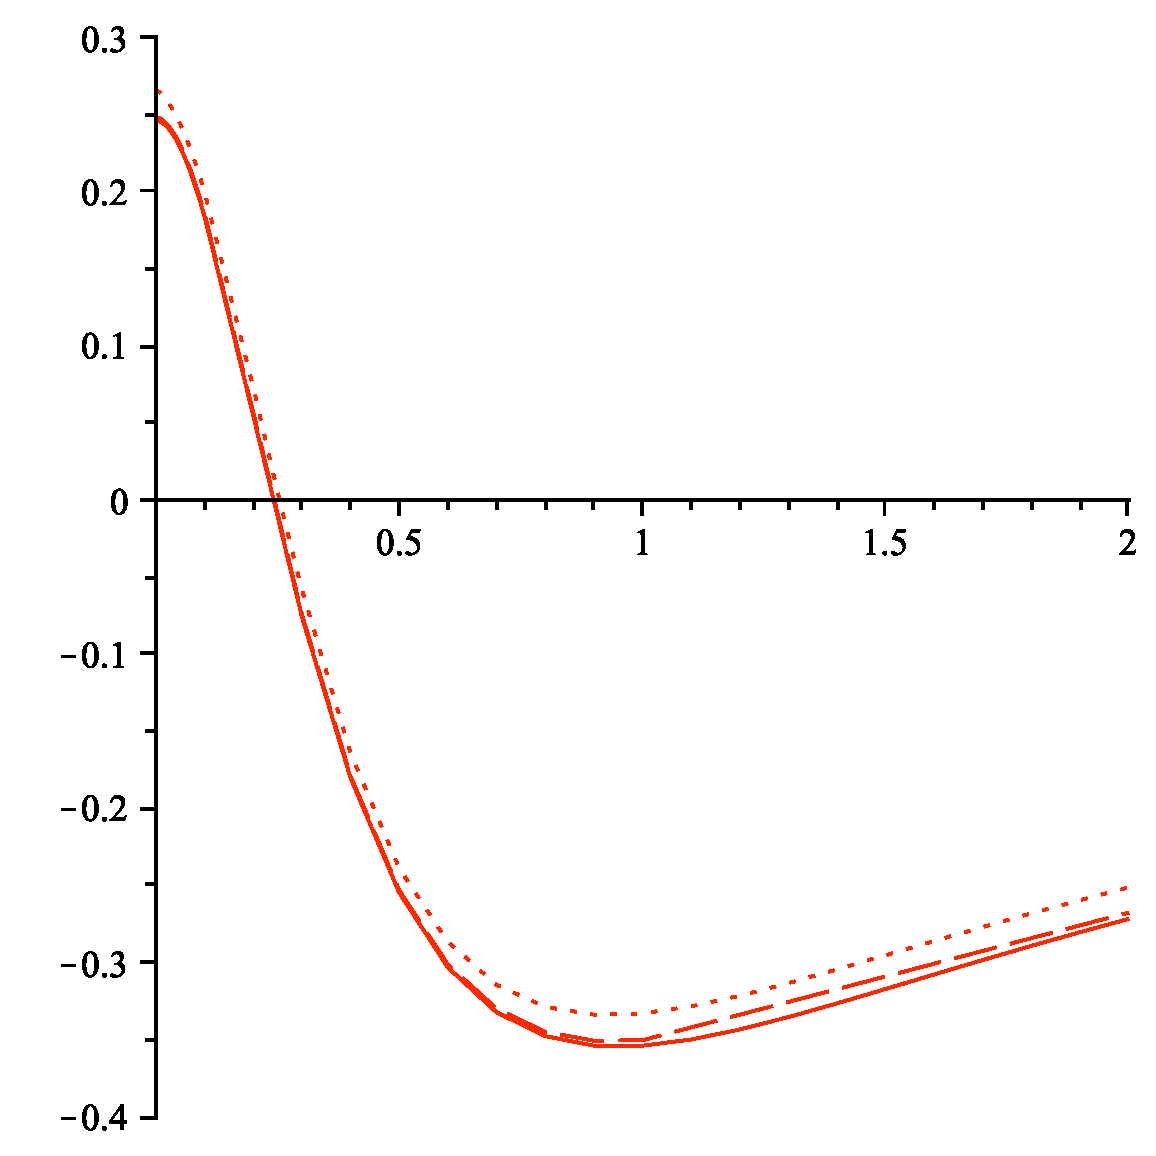
\includegraphics[scale=0.4]{images/graphics/Vacuum_Energy_2.pdf}\\
\small{$\kappa^\vac_\pt$ as a function of $\mpr \pt$\\
for $\N = 1$, $2$ and $3$ (dotted, dashed and solid lines)}
\end{center}
In $\mpr \pt = 0$, we have $\kappa^\vac_\pt \approx 0.266$, $0.248$ and $0.246$ for $\N = 1$, $2$ and $3$ respectively; as $\mpr \pt \to \infty$, we have $\kappa^\vac_\pt \to 0^-$. Since the result converges to an integral expression for $\N \to \infty$, I shall assume that the coefficients obtained by carrying out the computation for $\N = 3$ are already a good approximation.

This energy is represented by following Feynman diagram:
\begin{center}
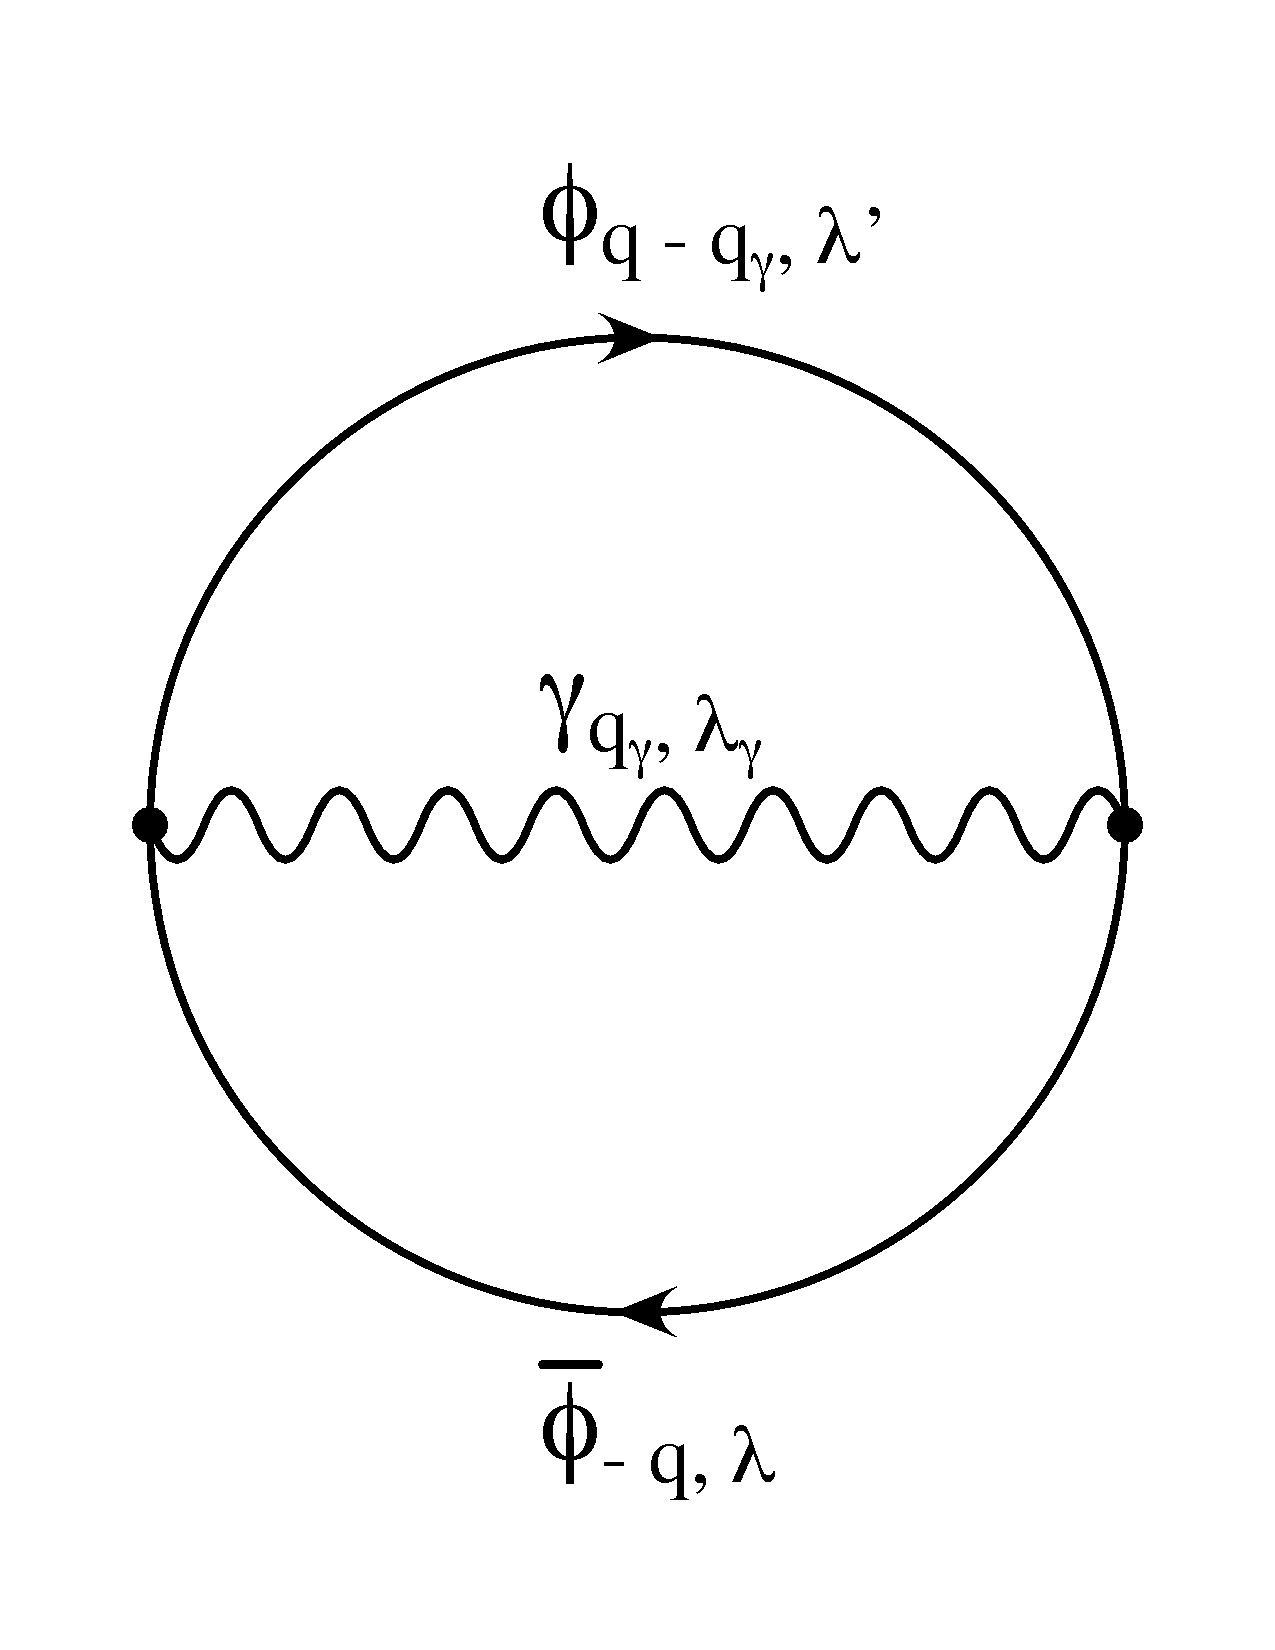
\includegraphics[scale=0.2]{images/diagrams/Vacuum_Energy_2.pdf}
\end{center}
where the Coulomb interaction term is conventionally  represented by the case $\sp_\photon = 0$.
Assuming $\kappa^\vac_\pt \approx 0.25$ for electrically charged fermions, the energy of the electromagnetically dressed vacuum evaluates up to the second order to:
\begin{equation*}
E^{(2)} \approx 0.25 ( 1 + 2 \N )^3 \frac {14} 3 \frac{\e^2}{4 \pi \vpty \a}
\end{equation*}

\section{Dressed charged fermion}

%TODO: Degenerate case! Correct formulas.

We consider an electrically charged fermion of type $\ptf$ in the bare state $\ket{\bQ 1 {\ptf} {\q_\ptf} {\sp_\ptf}}$. Up to the first order, the corresponding dressed state is composed of the bare state, of states of the form $\ket{\bQ 1 {\ptf} {\q_\ptf} {\sp_\ptf} \bQ 1 \pt {\eqp{\q-\q_\photon}} {\sp'} \bQ 1 {\antiparticle \pt} {-\q} \sp \bQ 1 \photon {\q_\photon} {\sp_\photon}}$, where $\pt$ is any electrically charged fermion, $\q_\photon \neq \sv 0$ and $(\pt, \q-\q_\photon, \sp') \neq (\ptf, \q_\ptf, \sp_\ptf)$, as well as of states of the form $\ket{\bQ 1 {\ptf} {\eqp{\q_\ptf - \q_\photon}} \sp \bQ 1 \photon {\q_\photon} {\sp_\photon}}$, where $\q_\photon \neq \sv 0$. The corresponding unnormalized coefficients  are given by:
\begin{equation*}
\FT \Phi^{(1)} = - \sqrt{\frac{\e^2}{4 \pi \vpty \h \c}} ( 1 + 2 \N )^{-3/2} \Qp \pt \frac{\ddirspin \pt {\q - \q_\photon} {\sp'} \gammat 0 \gamvec \dirspin {\antiparticle \pt} {-\q} \sp \ssp \cphotonspin {\q_\photon} {\sp_\photon}}{( 2 \pi q_\photon )^{1 / 2} \left( \Ek \pt {\q - \q_\photon} + \Ek {\antiparticle \pt} {-\q} + \Ek \photon {\q_\photon} \right) \a / \h \c}
\end{equation*}
for states of the form $\ket{\bQ 1 {\ptf} {\q_\ptf} {\sp_\ptf} \bQ 1 \pt {\eqp{\q-\q_\photon}} {\sp'} \bQ 1 {\antiparticle \pt} {-\q} \sp \bQ 1 \photon {\q_\photon} {\sp_\photon}}$, and by:
\begin{equation*}
\FT \Phi^{(1)} = - \sqrt{\frac{\e^2}{4 \pi \vpty \h \c}} ( 1 + 2 \N )^{-3/2} \Qp \ptf \frac{\ddirspin \ptf {\q_\ptf - \q_\photon} \sp \gammat 0 \gamvec \dirspin \ptf {\q_\ptf} {\sp_\ptf} \ssp \cphotonspin {\q_\photon} {\sp_\photon}}{( 2 \pi q_\photon )^{1 / 2} \left( \Ek \ptf {\q_\ptf - \q_\photon} + \Ek \photon {\q_\photon} - \Ek \ptf {\q_\ptf} \right) \a / \h \c}
\end{equation*}
for states of the form $\ket{\bQ 1 {\ptf} {\eqp{\q_\ptf - \q_\photon}} \sp \bQ 1 \photon {\q_\photon} {\sp_\photon}}$, respectively.

The corresponding energy is of second order and can be written as:
\begin{eqnarray*}
E^{(2)} & = & E^{(2)} \left( \vac \right) + \frac{\e^2}{4 \pi \vpty \a} \Qp \ptf^2 \kappa^\ptf_{\q_\ptf, \sp_\ptf} \\
\kappa^\ptf_{\q_\ptf, \sp_\ptf} & \eqdef & ( 1 + 2 \N )^{-3} \sum_{\q_\photon \neq \sv 0} \left[ \frac 1 {2 \pi q_\photon^2} \sum_\sp \left| \ddirspin \ptf {\q_\ptf - \q_\photon} \sp \dirspin \ptf {\q_\ptf} {\sp_\ptf} \right|^2 \right. \\
&& \left. - \frac {\sum_{\sp,\sp_\photon} \left| \ddirspin \ptf {\q_\ptf - \q_\photon} \sp \gammat 0 \gamvec \dirspin \ptf {\q_\ptf} {\sp_\ptf} \ssp \cphotonspin {\q_\photon} {\sp_\photon} \right|^2} {2 \pi q_\photon \left( \Ek \ptf {\q_\ptf - \q_\photon} + \Ek \photon {\q_\photon} - \Ek \ptf {\q_\ptf} \right) \a / \h \c} \right] \\
&& - ( 1 + 2 \N )^{-3} \sum_{\q_\photon \neq \sv 0} \left[ \frac 1 {2 \pi q_\photon^2} \sum_\sp \left| \ddirspin \ptf {\q_\ptf} {\sp_\ptf} \dirspin {\antiparticle \ptf} {-\q_\ptf - \q_\photon} \sp \right|^2 \right. \\
&& \left. - \frac {\sum_{\sp,\sp_\photon} \left| \ddirspin \ptf {\q_\ptf} {\sp_\ptf} \gammat 0 \gamvec \dirspin {\antiparticle \ptf} {-\q_\ptf - \q_\photon} \sp \ssp \cphotonspin {\q_\photon} {\sp_\photon} \right|^2} {2 \pi q_\photon \left( \Ek \ptf {\q_\ptf} + \Ek {\antiparticle \ptf} {-\q_\ptf - \q_\photon} + \Ek \photon {\q_\photon} \right) \a / \h \c} \right]
\end{eqnarray*}
where $E^{(2)} \left( \vac \right)$ is the second order energy of the dressed vacuum. The spin summations evaluate to:
\begin{eqnarray*}
\sum_{\sp} \left| \ddirspin \ptf {\q_\ptf - \q_\photon} \sp \dirspin \ptf {\q_\ptf} {\sp_\ptf} \right|^2 & = & \frac 1 2 \left( 1 + \frac{\mpr \ptf^2 + \eqp{\q_\ptf - \q_\photon} \ssp \q_\ptf}{\Ek \ptf {\q_\ptf - \q_\photon} \Ek \ptf {\q_\ptf} ( \a / \h \c )^2} \right) \\
\sum_{\sp,\sp_\photon} \left| \ddirspin \ptf {\q_\ptf - \q_\photon} \sp \gammat 0 \gamvec \dirspin \ptf {\q_\ptf} {\sp_\ptf} \ssp \cphotonspin {\q_\photon} {\sp_\photon} \right|^2 & = & 1 - \frac{\mpr \ptf^2 + ( \eqp{\q_\ptf - \q_\photon} \ssp \q_\photon ) ( \q_\ptf \ssp \q_\photon ) / q_\photon^2}{\Ek \ptf {\q_\ptf - \q_\photon} \Ek \ptf {\q_\ptf} ( \a / \h \c )^2} \\
\sum_{\sp} \left| \ddirspin \ptf {\q_\ptf} {\sp_\ptf} \dirspin {\antiparticle \ptf} {-\q_\ptf - \q_\photon} \sp \right|^2 & = & \frac 1 2 \left( 1 - \frac{\mpr \ptf^2 + \q_\ptf \ssp \eqp{\q_\ptf + \q_\photon}}{\Ek \ptf {\q_\ptf} \Ek {\antiparticle \ptf} {-\q_\ptf - \q_\photon} ( \a / \h \c )^2} \right) \\
\sum_{\sp,\sp_\photon} \left| \ddirspin \ptf {\q_\ptf} {\sp_\ptf} \gammat 0 \gamvec \dirspin {\antiparticle \ptf} {-\q_\ptf - \q_\photon} \sp \ssp \cphotonspin {\q_\photon} {\sp_\photon} \right|^2 & = & 1 + \frac{\mpr \ptf^2 + ( \q_\ptf \ssp \q_\photon ) ( \eqp{\q_\ptf + \q_\photon} \ssp \q_\photon ) / q_\photon^2}{\Ek \ptf {\q_\ptf} \Ek {\antiparticle \ptf} {- \q_\ptf - \q_\photon} ( \a / \h \c )^2}
\end{eqnarray*}
The vacuum energy diagram is also completed by subtracting following contribution:
\begin{center}
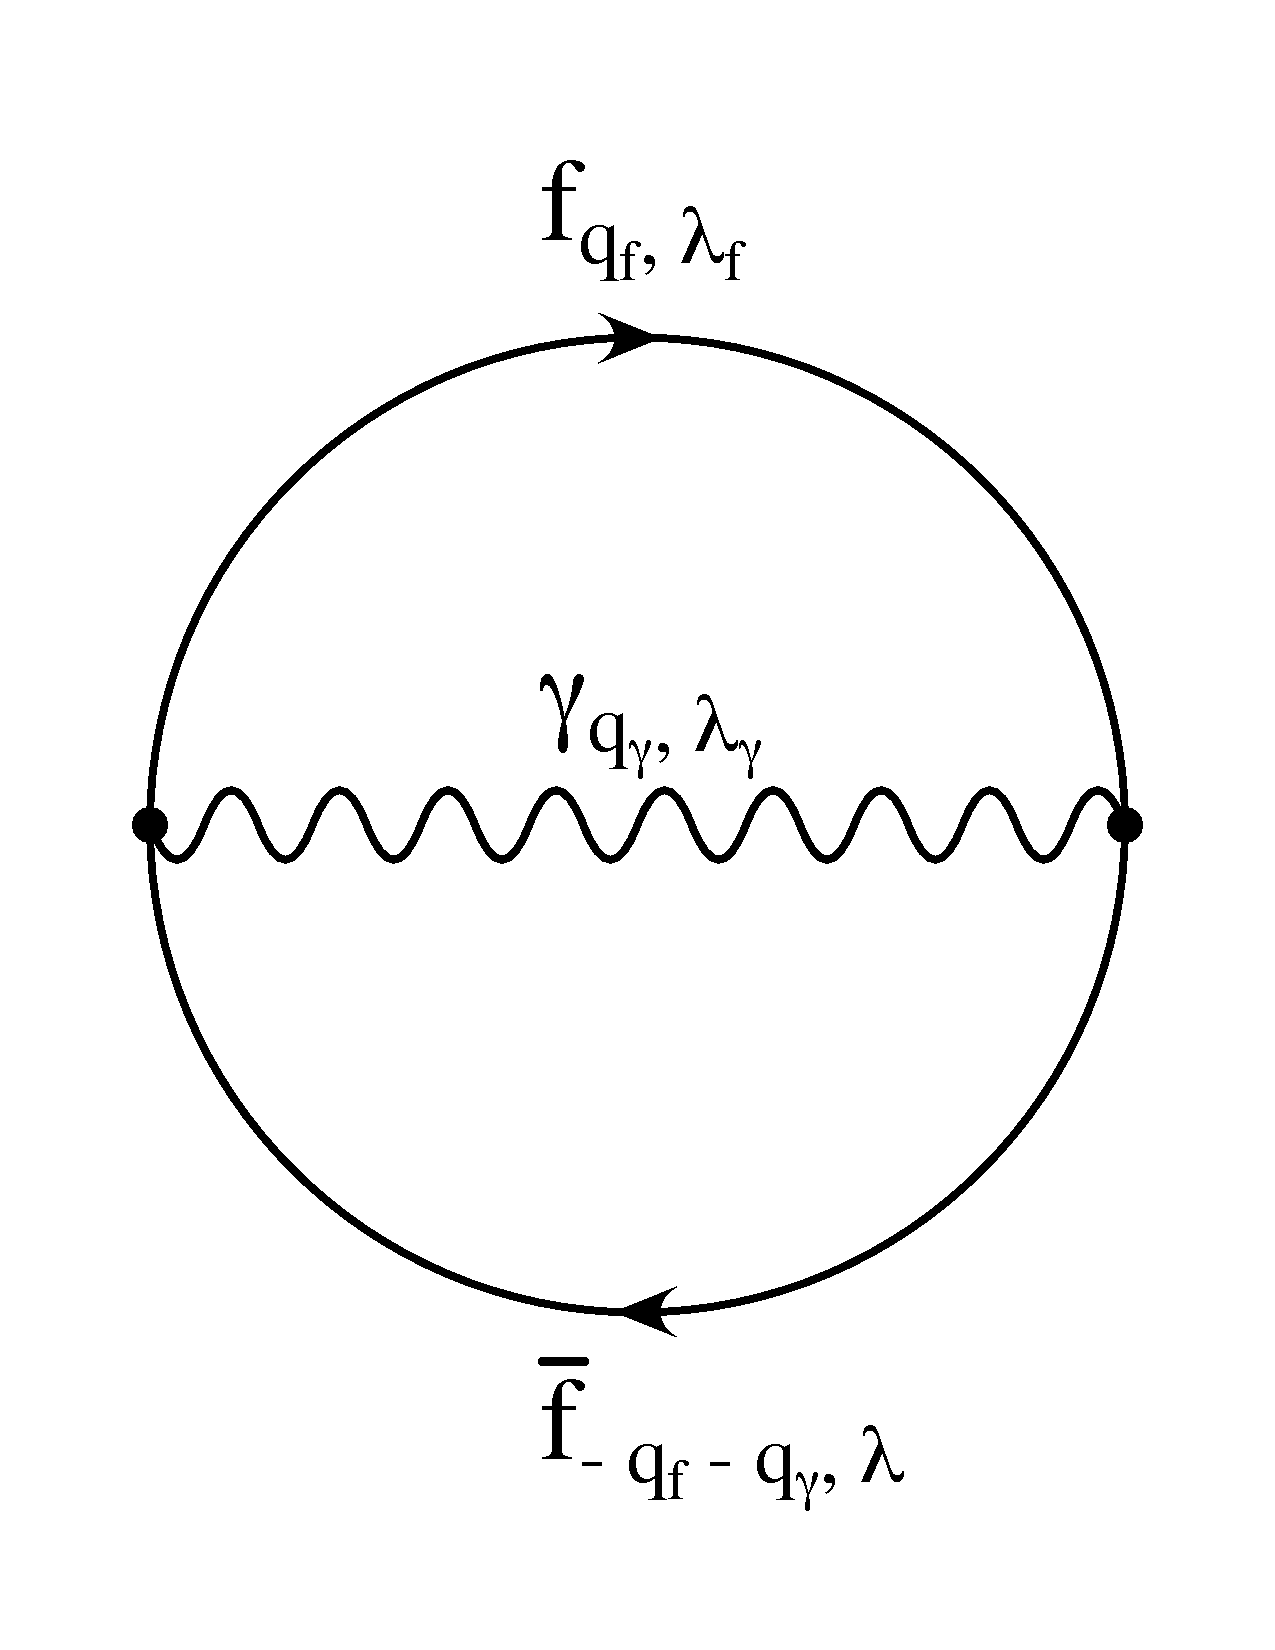
\includegraphics[scale=0.2]{images/diagrams/Charged_Fermion_Energy_2a.pdf}
\end{center}
and by adding following self-energy diagram:
\begin{center}
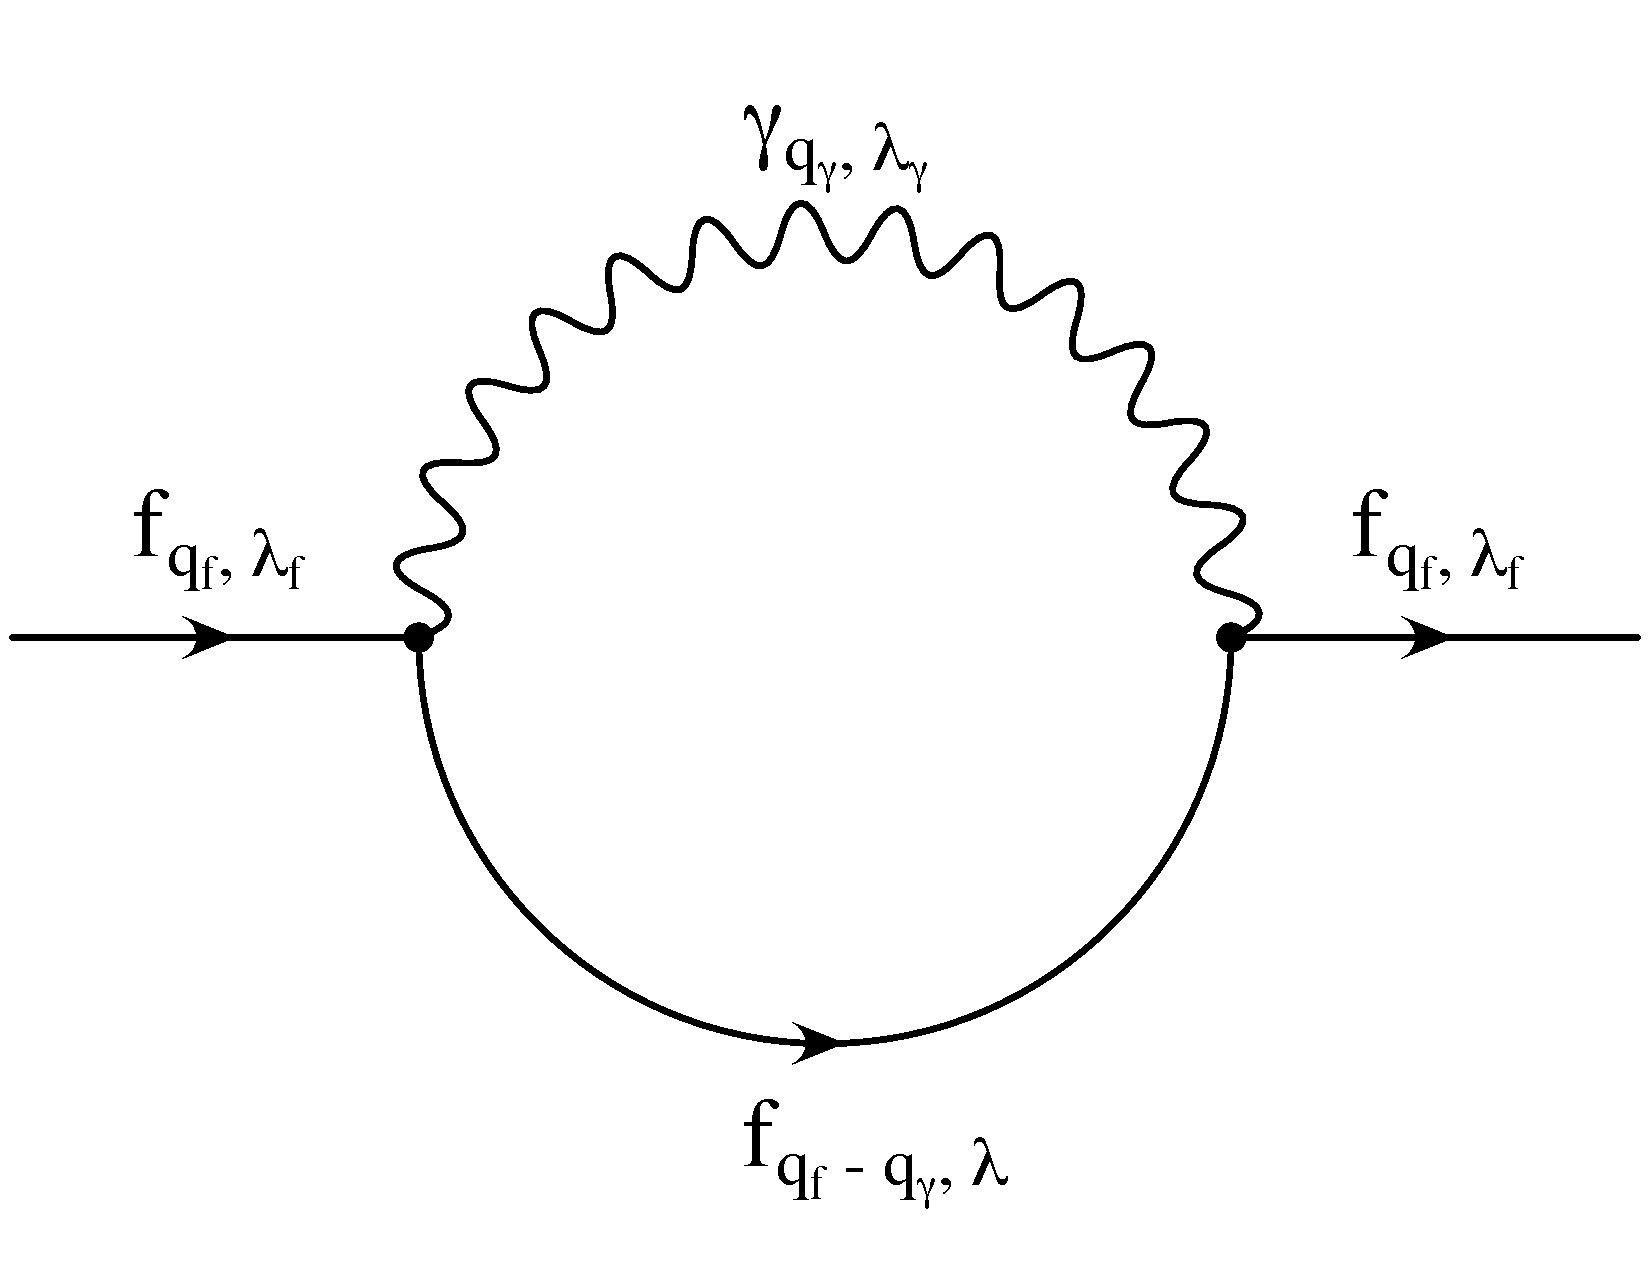
\includegraphics[scale=0.24]{images/diagrams/Charged_Fermion_Energy_2b.pdf}
\end{center}
for a given mode $(\q_\ptf, \sp_\ptf)$ of the fermion field.
%TODO: Evaluate at \q_\ptf = 0.

\section{Dressed photon}

We consider a photon in the bare state $\ket{\bQ 1 {\photon} {\q_ \photon} {\sp_ \photon}}$, where $\q_\photon \neq \sv 0$. Up to the first order, the corresponding dressed state is composed of the bare state, of states of the form $\ket{\bQ 1 {\photon} {\q_ \photon} {\sp_ \photon} \bQ 1 \pt {\eqp{\q-\q_\photon'}} {\sp'} \bQ 1 {\antiparticle \pt} {-\q} \sp \bQ 1 \photon {\q_\photon'} {\sp_\photon'}}$, where $\pt$ is any electrically charged fermion, $\q_\photon' \neq \sv 0$ and $(\q_\photon',\sp_\photon') \neq (\q_ \photon,\sp_ \photon)$, of states of the form $\ket{\bQ 2 {\photon} {\q_ \photon} {\sp_ \photon} \bQ 1 \pt {\eqp{\q-\q_\photon}} {\sp'} \bQ 1 {\antiparticle \pt} {-\q} \sp}$ as well as of states of the form $\ket{\bQ 1 {\pt} {\eqp{\q + \q_\photon}} {\sp'} \bQ 1 {\antiparticle \pt} {-\q} \sp}$. The corresponding unnormalized coefficients  are given by:
\begin{equation*}
\FT \Phi^{(1)} = - \sqrt{\frac{\e^2}{4 \pi \vpty \h \c}} ( 1 + 2 \N )^{-3/2} \Qp \pt \frac{\ddirspin \pt {\q - \q_\photon'} {\sp'} \gammat 0 \gamvec \dirspin {\antiparticle \pt} {-\q} \sp \ssp \cphotonspin {\q_\photon'} {\sp_\photon'}}{( 2 \pi q_\photon' )^{1 / 2} \left( \Ek \pt {\q - \q_\photon'} + \Ek {\antiparticle \pt} {-\q} + \Ek \photon {\q_\photon'} \right) \a / \h \c}
\end{equation*}
for states of the form $\ket{\bQ 1 {\photon} {\q_ \photon} {\sp_ \photon} \bQ 1 \pt {\eqp{\q-\q_\photon'}} {\sp'} \bQ 1 {\antiparticle \pt} {-\q} \sp \bQ 1 \photon {\q_\photon'} {\sp_\photon'}}$, by:
\begin{equation*}
\FT \Phi^{(1)} = - \sqrt{2 \frac{\e^2}{4 \pi \vpty \h \c}} ( 1 + 2 \N )^{-3/2} \Qp \pt \frac{\ddirspin \pt {\q - \q_\photon} {\sp'} \gammat 0 \gamvec \dirspin {\antiparticle \pt} {-\q} \sp \ssp \cphotonspin {\q_\photon} {\sp_\photon}}{( 2 \pi q_\photon )^{1 / 2} \left( \Ek \pt {\q - \q_\photon} + \Ek {\antiparticle \pt} {-\q} + \Ek \photon {\q_\photon} \right) \a / \h \c}
\end{equation*}
for states of the form $\ket{\bQ 2 {\photon} {\q_ \photon} {\sp_ \photon} \bQ 1 \pt {\eqp{\q-\q_\photon'}} {\sp'} \bQ 1 {\antiparticle \pt} {-\q} \sp}$, and by:
\begin{equation*}
\FT \Phi^{(1)} = - \sqrt{\frac{\e^2}{4 \pi \vpty \h \c}} ( 1 + 2 \N )^{-3/2} \Qp \pt \frac{\ddirspin \pt {\q + \q_\photon} {\sp'} \gammat 0 \gamvec \dirspin {\antiparticle \pt} {-\q} \sp \ssp \photonspin {\q_\photon} {\sp_\photon}}{( 2 \pi q_\photon )^{1 / 2} \left( \Ek \pt {\q + \q_\photon} + \Ek {\antiparticle \pt} {-\q} - \Ek \photon {\q_\photon} \right) \a / \h \c}
\end{equation*}
for states of the form $\ket{\bQ 1 {\pt} {\eqp{\q + \q_\photon}} {\sp'} \bQ 1 {\antiparticle \pt} {-\q} \sp}$, respectively.

The corresponding energy is of second order and can be written as:
\begin{eqnarray*}
E^{(2)} & = & E^{(2)} \left( \vac \right) - \frac{\e^2}{4 \pi \vpty \a} \sum_{\pt} \Qp \pt^2 \kappa^{\photon}_{\q_\photon,\sp_\photon,\pt} \\
\kappa^{\photon}_{\q_\photon,\sp_\photon,\pt} & \eqdef & ( 1 + 2 \N )^{-3} \sum_{\q} \frac {\sum_{\sp',\sp} \left| \ddirspin \pt {\q - \q_\photon} {\sp'} \gammat 0 \gamvec \dirspin {\antiparticle \pt} {-\q} \sp \ssp \cphotonspin {\q_\photon} {\sp_\photon} \right|^2} {2 \pi q_\photon \left( \Ek \pt {\q - \q_\photon} + \Ek {\antiparticle \pt} {-\q} + \Ek \photon {\q_\photon} \right) \a / \h \c} \\
&& + ( 1 + 2 \N )^{-3} \sum_{\q} \frac {\sum_{\sp',\sp} \left| \ddirspin \pt {\q + \q_\photon} {\sp'} \gammat 0 \gamvec \dirspin {\antiparticle \pt} {-\q} \sp \ssp \photonspin {\q_\photon} {\sp_\photon} \right|^2} {2 \pi q_\photon \left( \Ek \pt {\q + \q_\photon} + \Ek {\antiparticle \pt} {-\q} - \Ek \photon {\q_\photon} \right) \a / \h \c}
\end{eqnarray*}
where the spin summations evaluate to:
\begin{eqnarray*}
\sum_{\sp',\sp} \left| \ddirspin \pt {\q - \q_\photon} {\sp'} \gammat 0 \gamvec \dirspin {\antiparticle \pt} {-\q} \sp \ssp \cphotonspin {\q_\photon} {\sp_\photon} \right|^2 & = & 1 + \frac{\mpr \pt^2 + ( \eqp{\q - \q_\photon} \ssp \q_\photon ) ( \q \ssp \q_\photon ) / q_\photon^2}{\Ek \pt {\q - \q_\photon} \Ek {\antiparticle \pt} {-\q} ( \a / \h \c )^2} \\
\sum_{\sp',\sp} \left| \ddirspin \pt {\q + \q_\photon} {\sp'} \gammat 0 \gamvec \dirspin {\antiparticle \pt} {-\q} \sp \ssp \photonspin {\q_\photon} {\sp_\photon} \right|^2 & = & 1 + \frac{\mpr \pt^2 + ( \eqp{\q + \q_\photon} \ssp \q_\photon ) ( \q \ssp \q_\photon ) / q_\photon^2}{\Ek \pt {\q + \q_\photon} \Ek {\antiparticle \pt} {-\q} ( \a / \h \c )^2}
\end{eqnarray*}
The vacuum energy diagram is also completed by adding following (negative) contribution:
\begin{center}
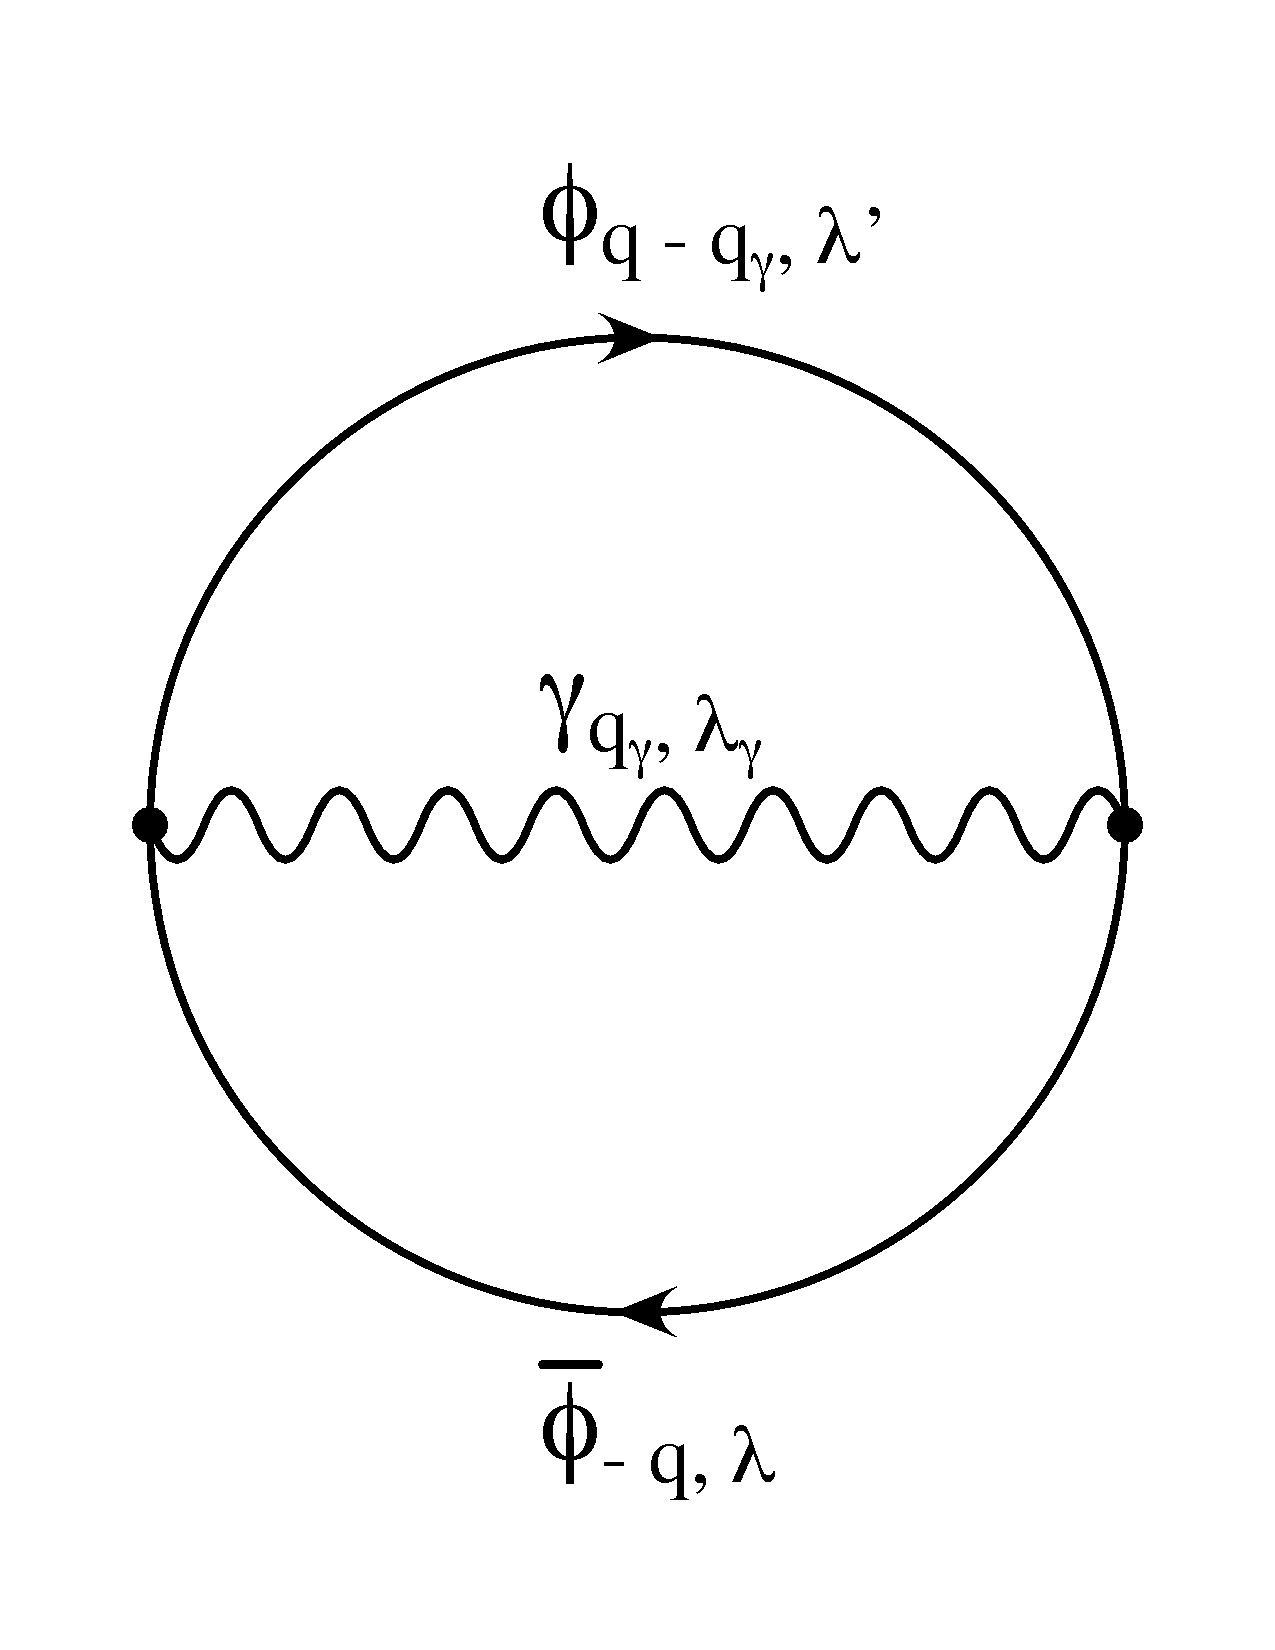
\includegraphics[scale=0.2]{images/diagrams/Photon_Energy_2a.pdf}
\end{center}
and by adding following (negative) self-energy diagram:
\begin{center}
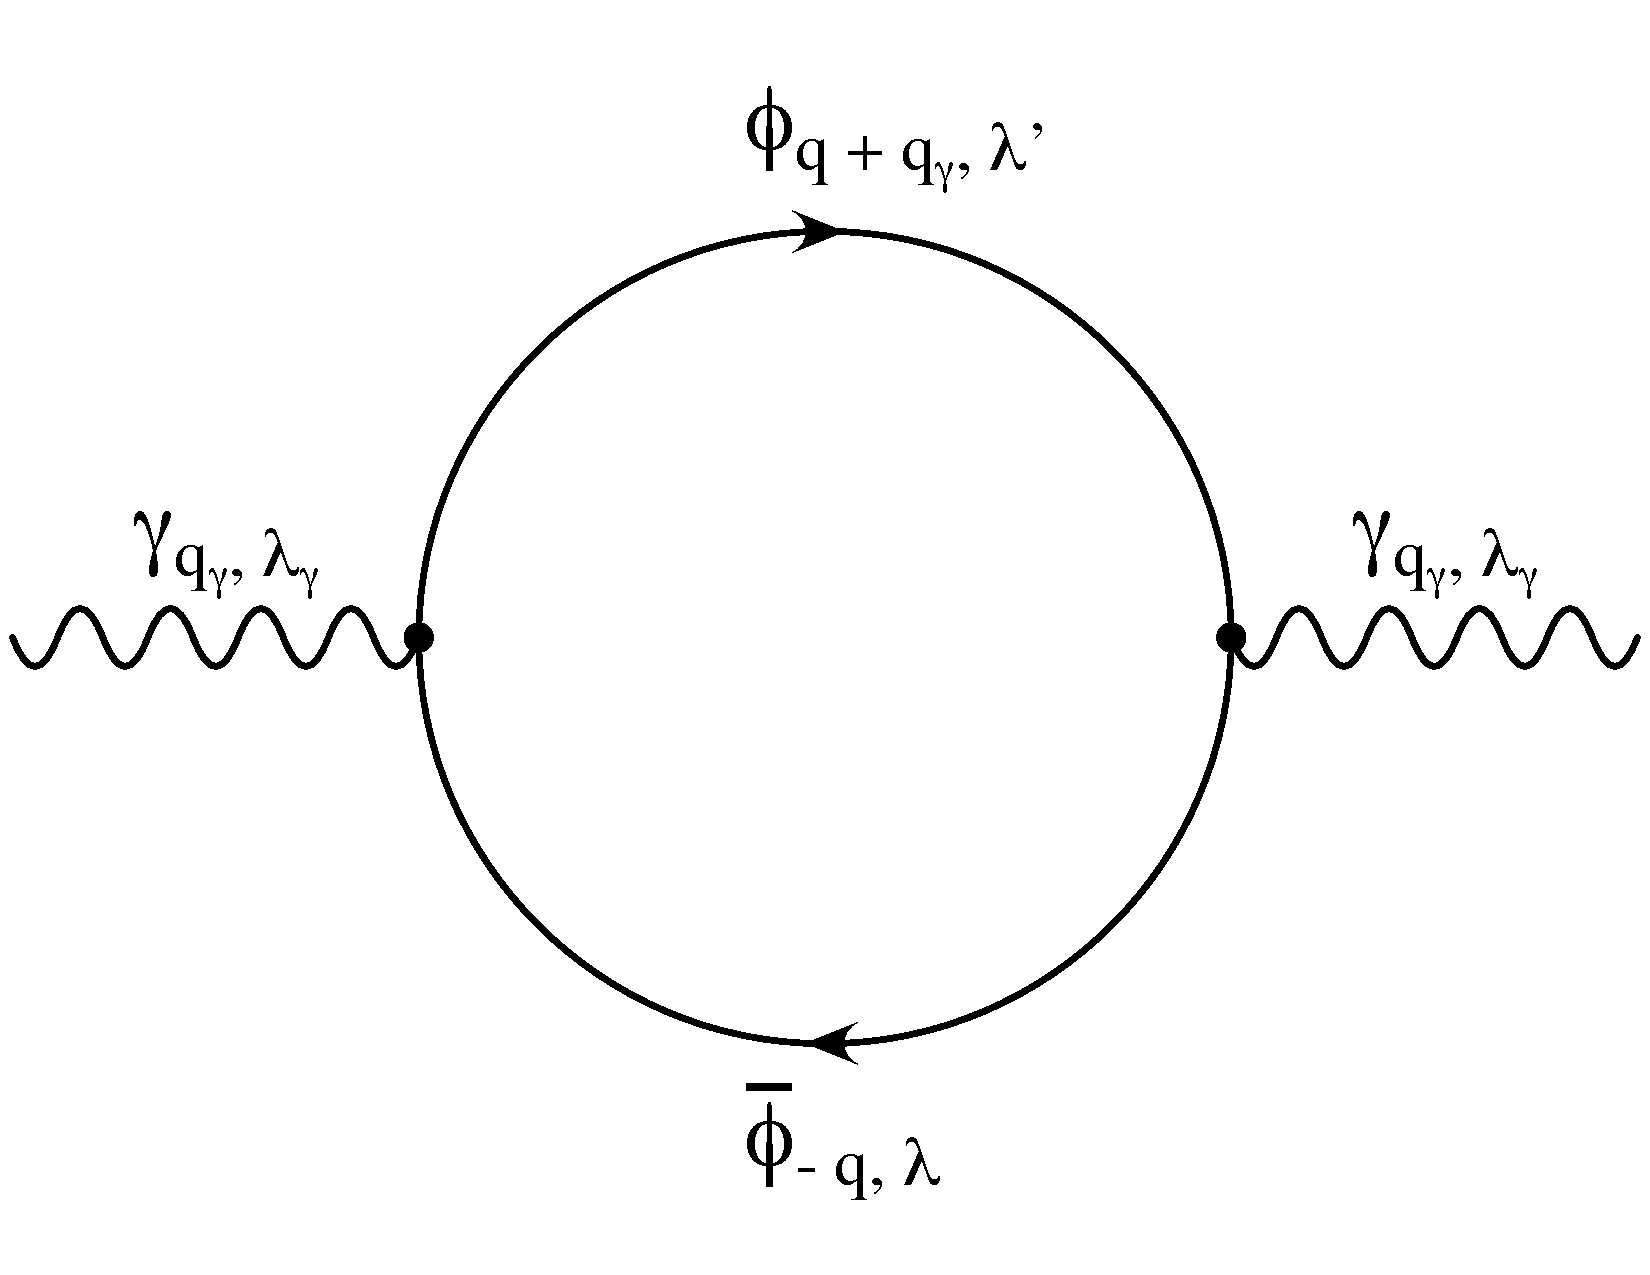
\includegraphics[scale=0.24]{images/diagrams/Photon_Energy_2b.pdf}
\end{center}
for a given mode $(\q_\photon, \sp_\photon)$ of the photon field.
